% Exercise Template
%A LaTeX template for typesetting exercise in Persian (with cover page).
%By: Reza Adinepour

\documentclass[12pt]{exam}

\usepackage{setspace}
\usepackage{listings}
\usepackage{graphicx,subfigure,wrapfig}
\usepackage{multirow}
\usepackage{matlab-prettifier}
\usepackage{amsmath}
\usepackage{multicol}


\usepackage[margin=20mm]{geometry}
\usepackage{xepersian}
\settextfont{XB Niloofar}

\newcommand{\class}{آزمایشگاه DSP}
\newcommand{\term}{نیم‌سال دوم ۰۱-۰۲}
\newcommand{\college}{دانشکده مهندسی برق}
\newcommand{\prof}{استاد: دکتر مقیمی}

\singlespacing
\parindent 0ex

\begin{document}


% -------------------------------------------------------
%  Thesis Information
% -------------------------------------------------------

\newcommand{\ThesisType}
{سمینار}  % پایان‌نامه / رساله
\newcommand{\ThesisDegree}
{کارشناسی ارشد گرایش معماری کامپیوتر}  % کارشناسی / کارشناسی ارشد / دکتری
\newcommand{\ThesisMajor}
{مهندسی برق}  % مهندسی کامپیوتر
\newcommand{\ThesisTitle}
{موضوع آزمایش}
\newcommand{\ThesisAuthor}
{رضا آدینه پور-9814303\\علی‌رضا قربانی-9823263}
\newcommand{\ThesisSupervisor}
{جناب آقای دکتر رضا خرقانیان}
\newcommand{\ThesisDate}
{اردی‌بهشت 1402}
\newcommand{\ThesisDepartment}
{دانشکده مهندسی برق}
\newcommand{\ThesisUniversity}
{دانشگاه صنعتی شاهرود}

% -------------------------------------------------------
%  English Information
% -------------------------------------------------------

\newcommand{\EnglishThesisTitle}{A Standard Template for Course Exercise}


\pagestyle{empty}

\begin{center}


\includegraphics[scale=0.17]{images/logo.png}

\vspace{0.5cm}
\ThesisUniversity \\[-0.3em]
\vspace{0.5cm}
\ThesisDepartment\\

\begin{large}
\vspace{0.5cm}


%\ThesisMajor

\end{large}

\vspace{1.5cm}

{عنوان:}\\[1.2em]
{\LARGE\textbf{\ThesisTitle}}\\ 
\vspace{1cm}
% \begin{latin}
% {\Large\textbf\EnglishThesisTitle}
% \end{latin}

\vspace{2cm}

{نگارش}\\[.5em]
{\large\textbf{\ThesisAuthor}}

\vspace{1.5cm}

{استاد مربوطه}\\[.5em]
{\large\textbf{\ThesisSupervisor}}

\vspace{1cm}



\vspace{2cm}

\ThesisDate

\end{center}

\newpage


% These commands set up the running header on the top of the exam pages
\pagestyle{head}
\firstpageheader{}{}{}
\runningheader{صفحه \thepage\ از \numpages}{}{\class}
\runningheadrule

\vspace{0pt}




\begin{questions}
\pointpoints{نمره}{نمره}

\question
با استفاده از متلب و بدون استفاده از توابع آماده مرتبط با SNR،‌تابعی بنویسید که یک سیگنال وعددی را به‌عنوان سیگنال به نویز از کاربر بگیرد و مقداری نویز به آن اضاف کند،‌به نحوی که خروجی تابع سیگنال نویزی شده با سیگنال به نویز مطلوب کاربر باشد.\\

• تابع نوشته شده به‌صورت زیر است: 
\begin{latin}
\begin{lstlisting}[
	frame=single,
	numbers=left,
	style=Matlab-editor %style: %Matlab-Pyglike, Matlab-bw
	] 
	
function noisy_signal = add_noise(signal, SNR)
	% Adds noise with a given SNR to a signal
	% signal: input signal
	% SNR: signal-to-noise ratio in dB
	
	% Calculate signal power
	signal_power = norm(signal)^2 / length(signal);
	
	% Calculate noise power from SNR
	noise_power = signal_power / (10^(SNR/10));
	
	% Generate noise with the same length as the signal
	noise = sqrt(noise_power) * randn(size(signal));
	
	% Add noise to the signal
	noisy_signal = signal + noise;
end

\end{lstlisting}
\end{latin}

\question
نهایتا با ایجاد یک تابع سینوسی و نویزی کردن آن با استفاده از تابع نوشته شده،‌کارایی تابع مذکور را برسی کنید. \\

• کد نوشته شده برای تست تابع به‌صورت زیر است: 
\begin{latin}
	\begin{lstlisting}[
		frame=single,
		numbers=left,
		style=Matlab-editor %style: %Matlab-Pyglike, Matlab-bw
		] 
		
clear; clc; close all;

% Generate a sine wave signal
Fs = 1000; % Sampling frequency
t = 0:1/Fs:1; % Time vector
f = 10; % Signal frequency
x = sin(2*pi*f*t); % Signal

% Add noise with SNR=5dB
SNR = input('Enter the desired SNR value: ');
noisy_signal = add_noise(x, SNR);

% Plot the original signal and the noisy signal
subplot(2,1,1);
plot(t,x);
title('Original signal');
grid on;
grid minor;

subplot(2,1,2);
plot(t,noisy_signal);
title(['Noisy signal with SNR =' num2str(SNR) 'dB']);
grid on;
grid minor;
		
\end{lstlisting}
\end{latin}

• خروجی برنامه یه‌صورت زیر است: 
\begin{figure}[h]
	\centering
	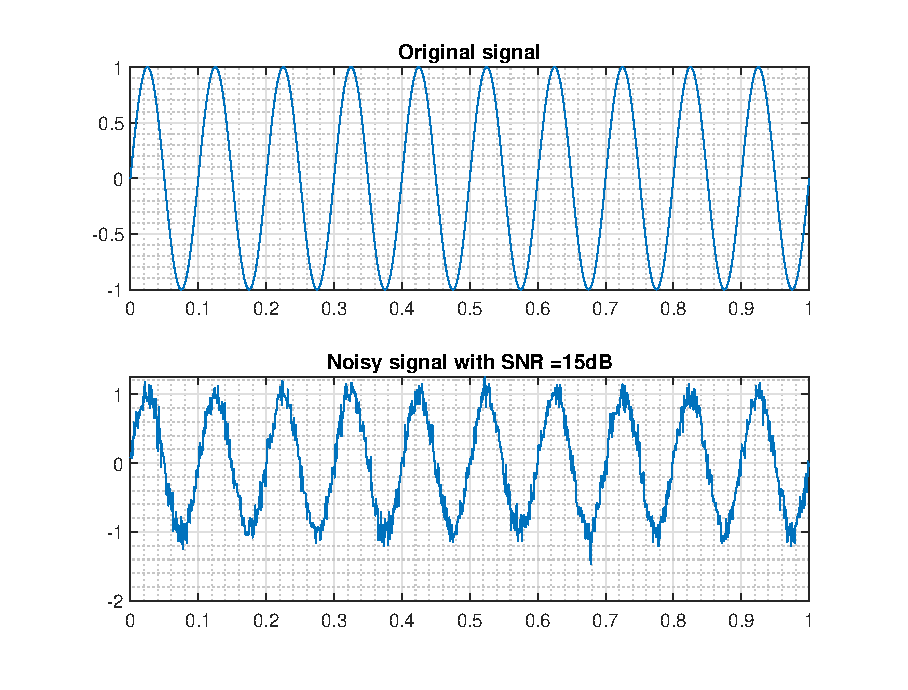
\includegraphics[width=1\textwidth]{images/Result}
	\caption{خروجی برنامه}
\end{figure}


\end{questions}
\end{document}

